\documentclass[12pt, letterpaper]{article}

% --- Preamble ---
\usepackage[backend=biber, style=numeric]{biblatex} 
\addbibresource{references.bib} % Make sure this file matches your .bib fil

%%%%%%%%%%%%%%%%%%%%%%%%%%%%%%%%%%%%%%%%%%%%%%%%%%%%
%%%%%%%%%%%%%%%% DO NOT MODIFY HERE %%%%%%%%%%%%%%%%
\usepackage[utf8]{inputenc}
\usepackage{graphicx} % Required for inserting images
\usepackage{mathrsfs}		 % For Symbols
\usepackage{amssymb}		 % For More Symbols
\usepackage{amsfonts}		 % For Other Symbols
\usepackage{amsmath}         % For Equations
\usepackage{mathtools}
\usepackage{amsthm}          % For Theorems & Definitions
\usepackage{tabularx}        % Package used to make variable width-columns, i.e.,
                             % column widths are changed to fit the maximum width
                             % and text is wrapped nicely.

\usepackage{threeparttable}

\usepackage{lscape}			% For landscape
\usepackage{adjustbox}		% To adjust table width
\usepackage{multirow}		% For merging and splitting table cells
\usepackage{float}          % For figure formatting
\usepackage{booktabs}       % For table formatting
\usepackage[parfill]{parskip}
\usepackage{hyperref}
\usepackage{lipsum}

%%%%%%%%%%%%%%%%%%%%%%%%%%%%%%%%%%%%%%%%%%%%%%%%%%%%
%%%%%%%%%%%%%%%%%%%%%%%%%%%%%%%%%%%%%%%%%%%%%%%%%%%%

%%%%%%%%%%%%%%%% MODIFY TITLE PAGE %%%%%%%%%%%%%%%%%
\title{3D Spherical Ring Attractor Network Documentation}
\author{Noah Ginzburg}
\date{\today}
%%%%%%%%%%%%%%%%%%%%%%%%%%%%%%%%%%%%%%%%%%%%%%%%%%%%


\begin{document}

\maketitle
\rule{0.95\textwidth}{0.5pt}

\tableofcontents
\newpage

%%%%%%%%%%%%%%%%%%%%%%%%%%%%%%%%%%%%%%%%%%%%%%%%%%%%
\section{Overview}

The goal of this project is to extend a 2D mean-field Ring Attractor Network (RAN) into a 3D spherical version for use on a Crazyflie drone for heading tracking. A ring attractor network is a recurrent neural network that forms a stable bump of activity which tracks sensory input. In 2D, nodes are placed on a ring and the network tracks a single angle. In 3D, nodes are placed on the surface of a sphere so that the network can represent a full heading direction in three-dimensional space \cite{salahshour2025allocentric}.

The network is governed by the following mean-field dynamics:

\begin{equation}
    \dot{z}_i = -z_i + \tanh\left(u \sum_j M_{ij} z_j + b_i - \beta\right) - \tanh(-\beta)
\end{equation}

where $z_i$ is the firing rate of node $i$, $u$ is the gain parameter, $M_{ij}$ is the connection kernel, $b_i$ is the external sensory input, and $\beta$ is a bias term. The network is integrated using Euler's method with timestep $dt$ [\textit{citation needed}].

The population vector average gives the decoded heading direction. In 3D, the node positions are converted to Cartesian coordinates, and the activation-weighted mean is computed as:

\begin{equation}
    \bar{\mathbf{v}} = \frac{\sum_i z_i \, \mathbf{p}_i}{\sum_i z_i}
\end{equation}

where $\mathbf{p}_i$ is the Cartesian unit vector for node $i$.

%%%%%%%%%%%%%%%%%%%%%%%%%%%%%%%%%%%%%%%%%%%%%%%%%%%%
\section{Generational of a Spherical Node Network}

\subsection{Node Placement: Fibonacci Sphere}

One approach to placing nodes on a sphere is the Fibonacci Sphere, which uses the golden ratio and Fibonacci spirals to generate nearly equidistant points. For $N$ points indexed $i = 0, 1, \ldots, N-1$:

\begin{equation}
    z_i = 1 - \frac{2i}{N-1}, \qquad r_i = \sqrt{1 - z_i^2}, \qquad \theta_i = i \cdot \frac{2\pi}{\varphi^2}
\end{equation}

where $\varphi = \frac{1+\sqrt{5}}{2}$ is the golden ratio. The main drawback is that nodes are generated asymmetrically, which produces an uneven connection kernel matrix $M$. While viable, further testing is needed to determine if the asymmetry of nodes causes a bias when the network is given identical targets to bifurcate between.

\subsection{Node Placement: Icosphere}

An icosphere is the only 3D sphere that can achieve near-perfectly equidistant points. It is recursively constructed using triangles starting from a base icosahedron with 12 vertices and 20 faces. Each subdivision level splits every triangle into 4 smaller triangles. The number of nodes at subdivision level $n$ is:

\begin{equation}
    N = 10 \cdot 4^n + 2
\end{equation}

This yields node counts of 12, 42, 162, 642, 2562, 10242, and so on. Because the icosphere has antipodal symmetry (for every node at position $\mathbf{p}$ there exists a node at $-\mathbf{p}$), the connection kernel is symmetric and heading tracking is uniform across all directions.

\subsection{Node Placement Comparison}
Both the Fibonacci Sphere and icosphere produce valid and usable spherical node networks. The icosphere was initially selected for its antipodal symmetry property due to ease of debugging. Further testing is required to determine the advantages and disadvantages of these methods, and whether one is more optimal or consistent given a specific performance metric.  

\subsection{Discretization Bias}

A fundamental limitation of any discrete node placement is that targets will not in general land exactly on a node [citation needed]. The sensory input at node $i$ from a target at angular distance $\alpha_i$ is:

\begin{equation}
    b_i = e^{\kappa(\cos \alpha_i - 1)} \cdot \gamma
\end{equation}

where $\kappa$ is a sharpness parameter and $\gamma$ is the target quality. The peak input for a given target occurs at the nearest node, at distance $d$:

\begin{equation}
    b_{\text{peak}} = e^{\kappa(\cos d - 1)}
\end{equation}

This function is strictly monotone decreasing in $d$, since $\frac{d}{dd}(\cos d - 1) = -\sin d < 0$ for $d \in (0, \pi)$. Therefore:

\begin{equation}
    d_A < d_B \implies b_{\text{peak}}^A > b_{\text{peak}}^B
\end{equation}

A target that happens to land closer to a node receives a stronger peak input than one that falls between nodes. With winner-take-all dynamics above the critical gain $u_{\text{crit}}$, even small differences in peak input are amplified by the nonlinear dynamics, causing the closer target to be selected more often than 50\% of the time. The only clean solution is to increase resolution (larger $n$), which shrinks the maximum node-to-target gap.

\subsection{Further Generation Ideas}
One could represent the spherical node network using a spherical Fourier series. A spherical FFT converts the network state between the spatial representation, activity per node, and the spectral representation, coefficients of a spherical harmonic expansion. One would then manipulate the Fourier coefficients to achieve the node activations that result from network dynamics. This reduces the cost of the coupling step and removes the need for a uniform node distribution, since the representation is continuous rather than sampled. This idea significantly deviates from the original research basis of a network of neurons, however, it is worth mentioning for future research exploration potential.


%%%%%%%%%%%%%%%%%%%%%%%%%%%%%%%%%%%%%%%%%%%%%%%%%%%%
\section{Methods}

\subsection{Coordinate Convention}

Nodes are stored internally in polar coordinates as $(r, \phi, \theta)$ where $\phi \in [-\pi, \pi]$ is the azimuthal angle in the $xy$-plane and $\theta \in [0, \pi]$ is the polar angle from the $z$-axis (colatitude). Array indices are defined as:

\begin{equation}
    \text{MAG} = 0, \qquad \text{PHI} = 1, \qquad \text{THETA} = 2
\end{equation}

\subsection{Geodesic Distance}

The angular distance between two points on a unit sphere is computed using the spherical law of cosines \cite{bressloff2019stochastic}:

\begin{equation}
    \alpha = \arccos\left(\cos\theta_i \cos\theta_j + \sin\theta_i \sin\theta_j \cos(\phi_i - \phi_j)\right)
\end{equation}

The argument is clipped to $[-1, 1]$ to avoid numerical errors from floating point values slightly outside the domain of $\arccos$, e.g. $\arccos(1.0004)$.

\subsection{Connection Kernel}

The connection weight between nodes $i$ and $j$ is:

\begin{equation}
    M_{ij} = \cos\!\left(\pi \left(\frac{\alpha_{ij}}{\pi}\right)^v\right) \cdot \frac{1}{N}
\end{equation}

where $\alpha_{ij}$ is the geodesic distance between nodes $i$ and $j$,e $J$ is the kernel amplitude scalar, $v$ controls the kernel shape (sharpness of the Von-Mises distribution profile), and $N$ is the total number of nodes. The $1/N$ normalization ensures that the maximum eigenvalue of $M$ remains approximately constant as $N$ increases, keeping $u_{\text{crit}}$ stable across resolutions. 

This equation was not modified from the current literature of 2D ring attractor networks that use mean-field dynamics [cite Sindiso]. However, in the implementation, a scalar factor of $J$ was added to this equation for fine-tuning the amplitude of kernel. The inspiration came from the \textit{Stochastic neural field theory of wandering bumps on a sphere} paper by Paul C. Bresseloff, which provided helpful equations for an attractor network on a sphere. They use a cosine shaped curve with the following formula \cite{bressloff2019stochastic}: 

\begin{equation}
        J(\theta, \phi \mid \theta', \phi') = J_0 + J \left[ \cos\theta \cos\theta' + \sin\theta \sin\theta' \cos(\phi - \phi') \right]
\end{equation}

The resulting decision was to stay with the Von-Mises distribution shape to adhere to the current literature [cite Sindiso].

\subsection{Critical Gain}
 The critical gain $u_{\text{crit}}$ is the value of the coupling parameter where a spontaneous bump emerges. Below this value, the state is stable, so noise decays and nothing forms. Above it, the dominant mode has a positive growth rate, so any perturbation gets amplified into a bump. Currently, empirical tuning via parameter sweeps is the only way to accurately determine this value. One must generate the SAN in the presence of zero targets for different $u$ values until the normalized activation values become non-zero. Further research is necessary to determine if there is a reliable mathematical method to calculate this value based on given network parameters.

\subsection{Sensory Input}

The external input vector $\mathbf{b}$ is generated from a list of targets. Each target is defined by $(r, \phi, \theta, \gamma)$ where $\gamma$ is quality (signal strength). The input at node $i$ summed over all targets is:

\begin{equation}
    b_i = \frac{1}{\sqrt{N}} \sum_j \gamma_j \, e^{\kappa(\cos \alpha_{ij} - 1)}
\end{equation}

where $\alpha_{ij}$ is the geodesic distance from node $i$ to target $j$.  

\subsection{Integration}

The network is integrated with Euler's method including additive Gaussian noise:

\begin{equation}
    z(t + dt) = z(t) + dt \left(-z + \tanh(u M z + b - \beta) - \tanh(-\beta)\right) + \eta
\end{equation}

where $\eta \sim \mathcal{N}(0, \sigma\sqrt{dt}/\sqrt{N})$ per node. Noise is required for symmetry breaking when two targets are of equal quality and equidistant. Note that the dynamics remain identical to the original ring attractor network, only the shape of the network changed when transitioning to a 3D network.

\subsection{Computational Cost}

The dominant cost per integration step is the matrix-vector product $Mz$, which requires $\mathcal{O}(N^2)$ operations. At 50 Hz (20 ms per step) with NumPy Basic Linear Algebra Subprograms (BLAS), the practical resolution limits are approximately:

\begin{itemize}
    \item Modern laptop: up to $n = 5$ ($N = 10{,}242$ nodes)
    \item Raspberry Pi 4: up to $n = 3$ to $n = 4$ ($N = 642$ to $2{,}562$ nodes)
\end{itemize}

A modern laptop CPU (Intel i7/i9 or Apple M-series) doing numpy BLAS matrix operations achieves roughly 50 Giga floating point operations per second (GFLOPS) in practice. A Raspberry Pi 4 has a Cortex-A72 ARM CPU which is roughly 10 to 20 times slower than a laptop for this kind of workload. These are well-known ballpark figures.

For exampple, if you have a budget of 20ms per step at 50Hz. The cost of M @ z is $2N^2$ FLOPS. So:

$$\frac{2N^2}{\text{GFLOPS} \times 10^9} \leq 0.02$$

Solve for $N$:

$$N \leq \sqrt{\frac{0.02 \times \text{GFLOPS} \times 10^9}{2}}$$

For a laptop at 50 GFLOPS:

$$N \leq \sqrt{\frac{0.02 \times 50 \times 10^9}{2}} = \sqrt{5 \times 10^8} \approx 22{,}000$$

Then, use the icosphere subdivision level provides $N$ below that limit. Note that this does not take into account the processing power required to run additional software components such as a simulator.


%%%%%%%%%%%%%%%%%%%%%%%%%%%%%%%%%%%%%%%%%%%%%%%%%%%%
\section{Results}
\subsection{Parameters}
The following parameters were used to generate the results below unless otherwise stated: 

\begin{verbatim}
    nsub  = 3                  # N_s = 642 nodes
    N_s   = 10 * 4**nsub +2
    beta = 1.5
    v = 0.5
    dt = 0.1
    sigma = 1.5
    kappa = 5.0    
    u = 32.0
\end{verbatim}

\subsection{Kernel Generation}
Using the code in Section \ref{AppendixA}, the kernel was generated and plotted for an icosphere with $N = 642$ nodes. Figure \ref{fig:kernelShape} shows the shape of the kernel by overlaying the connection strengths between every pair of nodes as a function of geodesic distance. The connection strength decreases monotonically from a maximum of $1/N \approx 0.0016$ at $\alpha = 0$ to a minimum of $-1/N \approx -0.0016$ at $\alpha = \pi$, so nearby nodes excite each other and distant nodes inhibit each other. Since no additional amplitude scaling was applied, the kernel bounds are set entirely by the $1/N$ normalization. The kernel crosses zero where $(\alpha/\pi)^v = 1/2$, i.e. at $\alpha_0 = \pi \cdot 2^{-1/v}$, which is $\alpha_0 = \pi/4$ for $v = 0.5$.

\begin{figure}[H]
    \centering
    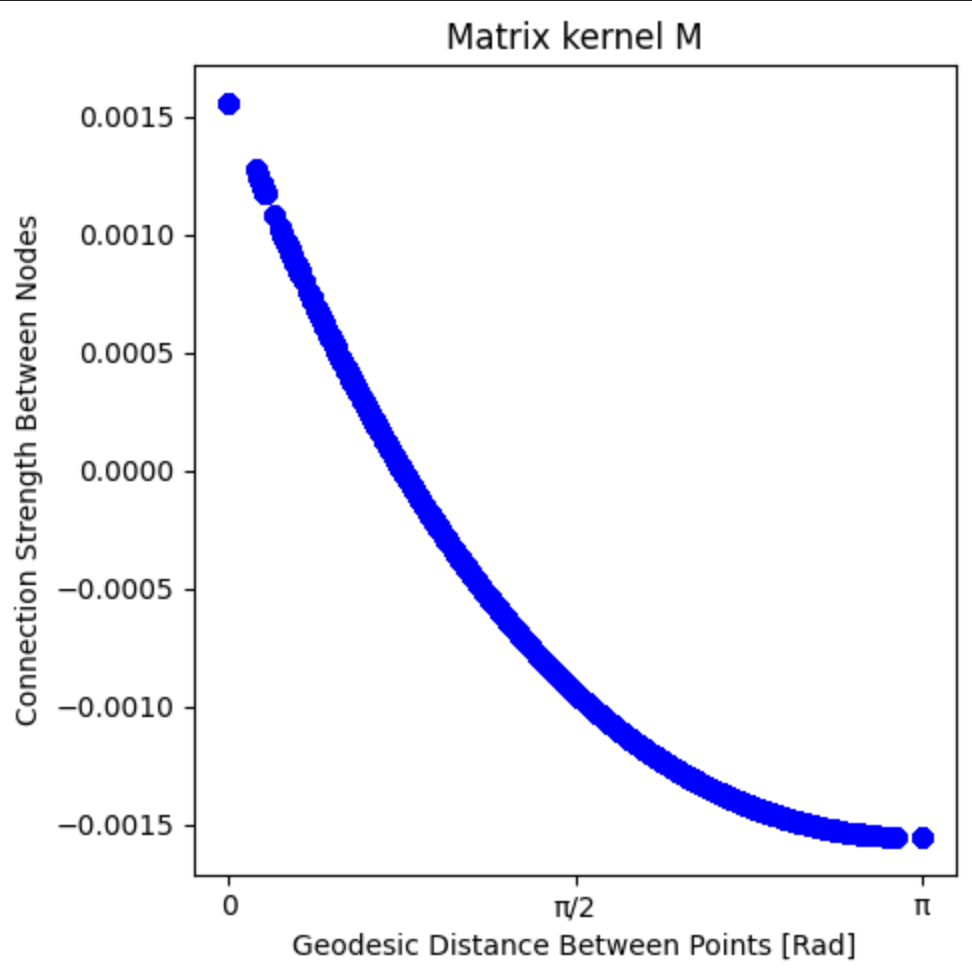
\includegraphics[width=0.5\linewidth]{RAN/RAN_Progress/newer_photos/M_Shape.png}
    \caption{Plot of connection strength of kernel $M$ vs. geodesic distance between points ($N = 642$, $v = 0.5$). The kernel is shaped as described by the Von-Mises distribution equation and is bounded by $\pm 1/N$.}
    \label{fig:kernelShape}
\end{figure}

Figure \ref{fig:kernelHeatmap} shows the row of $M$ belonging to a reference node on the equator ($\phi = 0$, $\theta = \pi/2$, marked with a star), plotted over $\theta$ vs. $\phi$ for $v = 0.3$, $0.4$, $0.5$, and $0.6$. The excitatory (red) region around the reference node is circular and isotropic, confirming that the kernel depends only on geodesic distance and not on direction. Increasing $v$ widens the excitatory region, with the zero crossing moving from $\alpha_0 \approx 0.31$ rad at $v = 0.3$ to $\alpha_0 \approx 0.99$ rad at $v = 0.6$, while the inhibitory (blue) region shrinks correspondingly. The peak and trough values remain fixed at $\pm 1/N$ for all $v$. A wider excitatory region produces a wider activity bump, so $v$ directly sets the bump width of the network.

\begin{figure}[H]
    \centering
    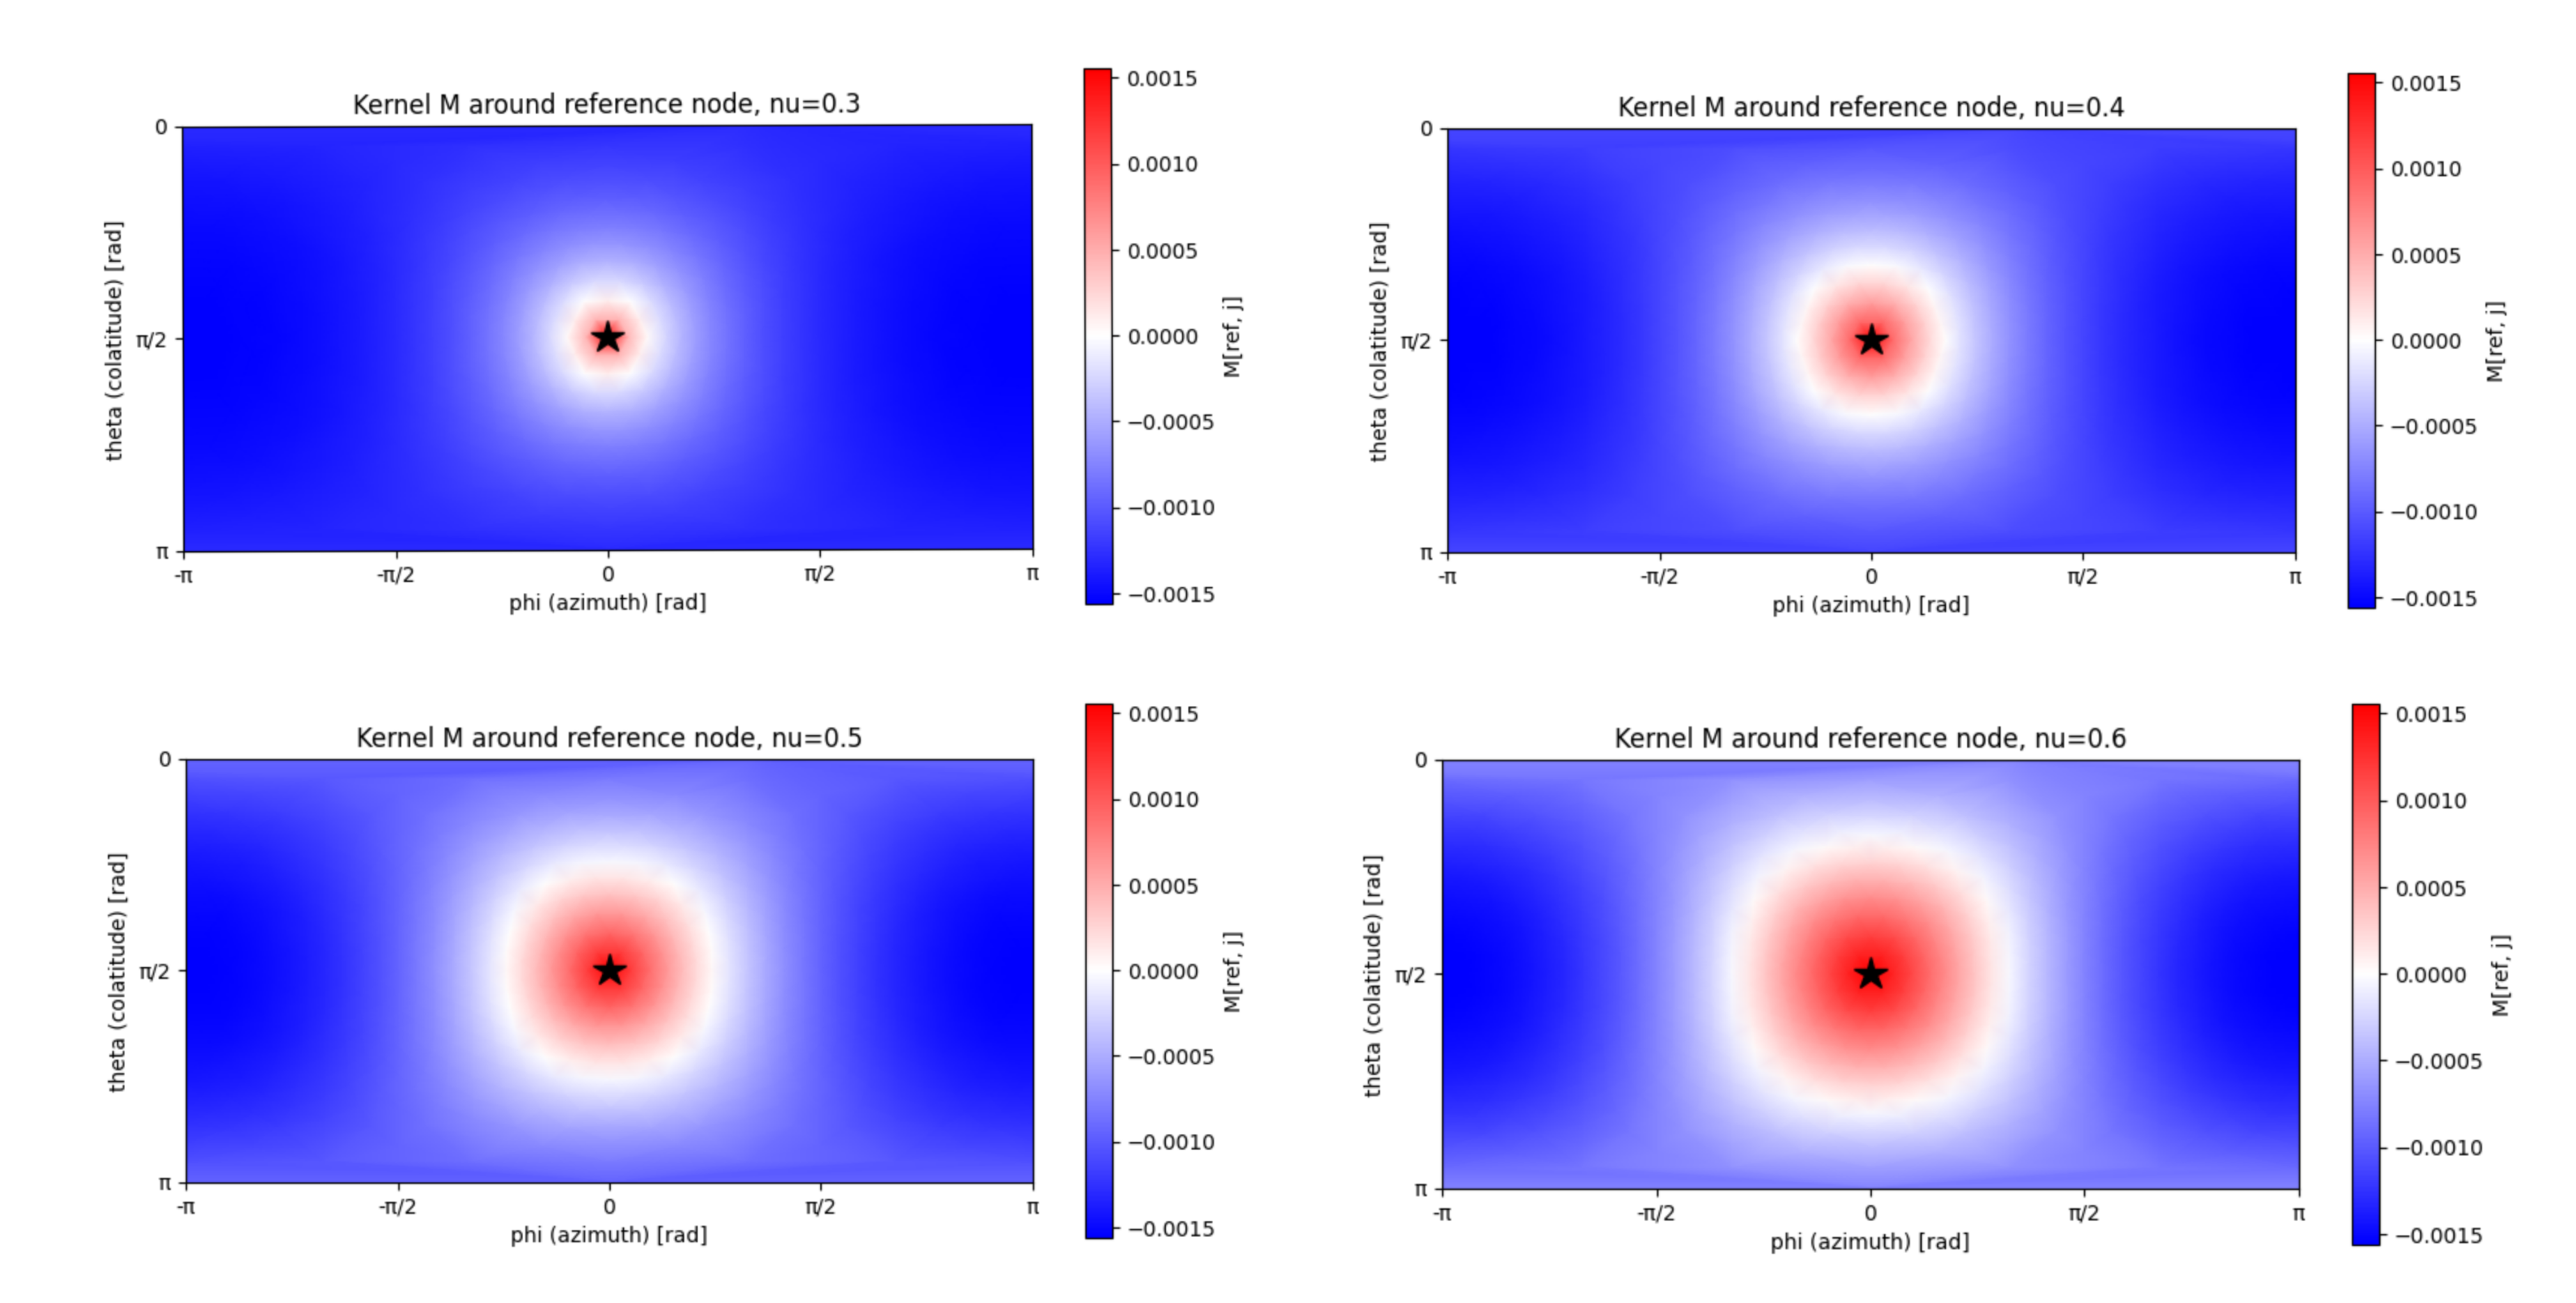
\includegraphics[width=1\linewidth]{RAN/RAN_Progress/newer_photos/M_HeatmapCombined.png}
    \caption{Kernel matrix $M$ around a reference node (star) plotted over $\theta$ (colatitude) vs. $\phi$ (azimuth) for $v = 0.3, 0.4, 0.5, 0.6$. Red indicates excitatory connections and blue indicates inhibitory connections.}
    \label{fig:kernelHeatmap}
\end{figure}

\subsection{Finding Critical Gain}
Using the parameters stated earlier, all targets were deactivated and a parameter sweep was run over $u = 0$ to $u = 69$ in steps of 1. For each $u$ value, 10 trials of $T = 300$ timesteps were run with $\sigma = 0.5$, and the norm of the final activation vector $\|z\|$ was recorded. Figure \ref{fig:zvu} shows the mean $\|z\|$ for each $u$ value, with error bars showing one standard deviation across trials.

\begin{figure}[H]
    \centering
    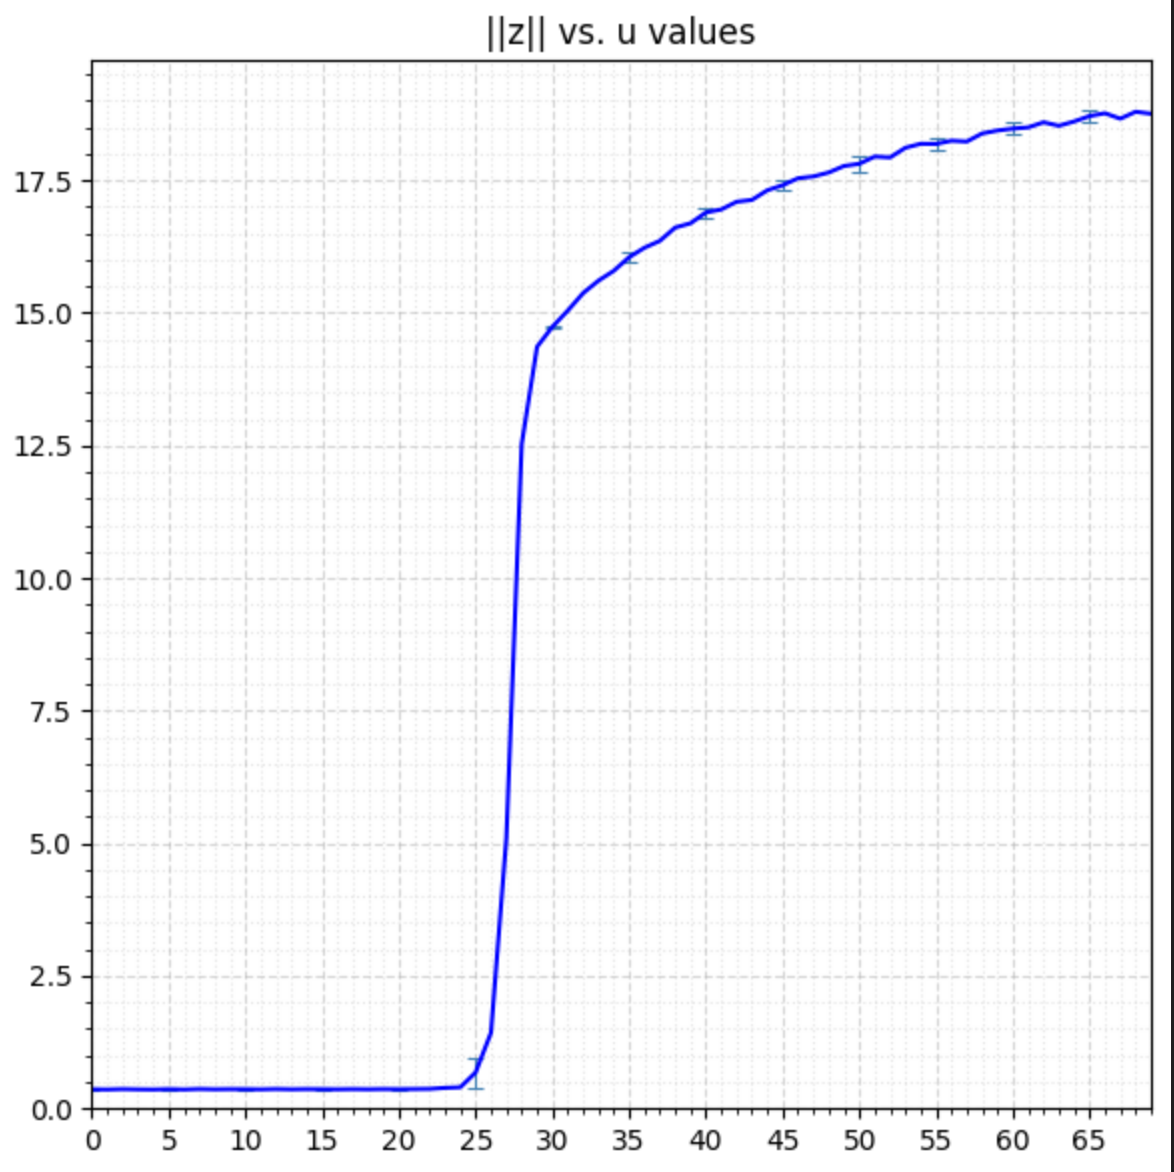
\includegraphics[width=0.6\linewidth]{RAN/RAN_Progress/newer_photos/zvsu.png}
    \caption{Plot of activation norm $\|z\|$ vs. $u$ with zero targets ($N = 642$, 10 trials per $u$). A spontaneous bump forms around $u_c \approx 26$.}
    \label{fig:zvu}
\end{figure}

Below $u \approx 24$, $\|z\|$ stays at the noise floor of approximately $0.4$, meaning noise decays and no bump forms. Between $u = 25$ and $u = 29$, $\|z\|$ jumps sharply to approximately $14.5$, marking the critical gain at $u_c \approx 26$. The larger error bar at $u = 25$ reflects that, near the transition, only some trials form a bump. Above the transition, $\|z\|$ continues to grow slowly and saturates near $19$ as the $\tanh$ nonlinearity limits the activation of each node. The operating value of $u = 32$ was chosen to sit just above this transition, so that the network reliably forms a bump without being driven deep into saturation.

\subsection{Single Target Tracking}

With a single target, the network correctly forms a single activity bump centered on the target location. The population vector average accurately recovers the target direction. Figure \ref{fig:one_targ_plot} shows a surface plot of the sensory input from the target (left) and a surface plot of the resulting RAN activation (right) over $\phi$ and $\theta$. The recurrent dynamics amplify the input into a stable, saturated bump directly over the target, with a peak activation considerably larger than the peak input.

\begin{figure}[H]
    \centering
    \begin{minipage}{0.48\linewidth}
        \centering
        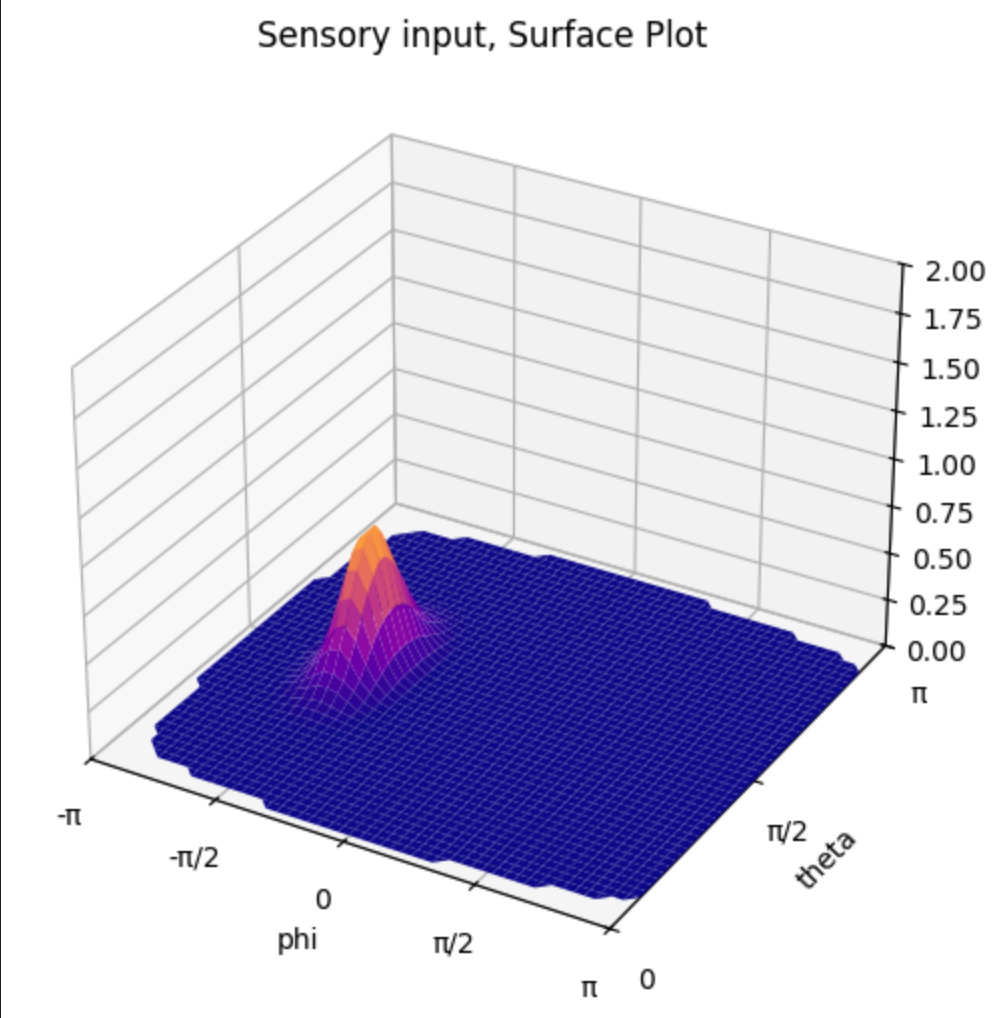
\includegraphics[width=\linewidth]{RAN/RAN_Progress/newer_photos/1_targ_input.png}
    \end{minipage}\hfill
    \begin{minipage}{0.48\linewidth}
        \centering
        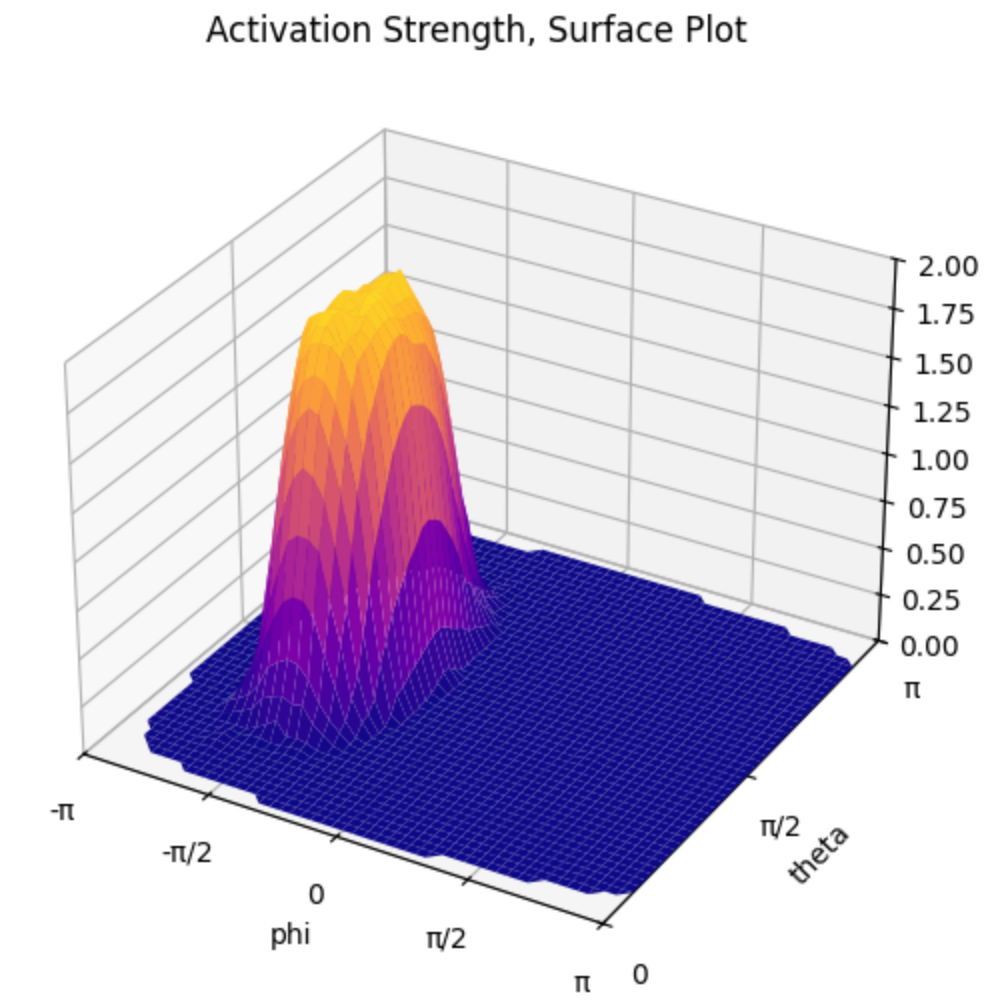
\includegraphics[width=\linewidth]{RAN/RAN_Progress/newer_photos/1_targ_bump.png}
    \end{minipage}
    \caption{Surface plots of sensory input (left) and resulting RAN activation strength (right) for one target. A stable bump forms over the target.}
    \label{fig:one_targ_plot}
\end{figure}

\subsection{Two Target Selection with Equal Qualities}

With two targets that have equal qualities, the network exhibits winner-take-all behavior above $u_{\text{crit}}$. When targets are placed 180 degrees apart (antipodal), selection is 50/50 due to noise-driven symmetry breaking. For non-antipodal targets, discretization bias causes the target closer to a node to be selected more frequently. For the following figures, both targets were given quality $\gamma = 20$ and placed at $\theta = \pi/2$, with one at $\phi = 0$ and the other at $\phi = \pi$. Both these angle combinations align perfectly with an icosphere node, thus, no discretization bias is present. Figure \ref{fig:two_targ_plot} shows a surface plot of the sensory input from both targets (left) and the resulting RAN activation (right). Note that the target at $\phi = \pi$ appears split across the left and right edges of the input plot because $\phi = -\pi$ and $\phi = \pi$ are the same direction. The network suppresses the input from one target entirely and forms a single stable bump over the other, randomly-selected target.

\begin{figure}[H]
    \centering
    \begin{minipage}{0.48\linewidth}
        \centering
        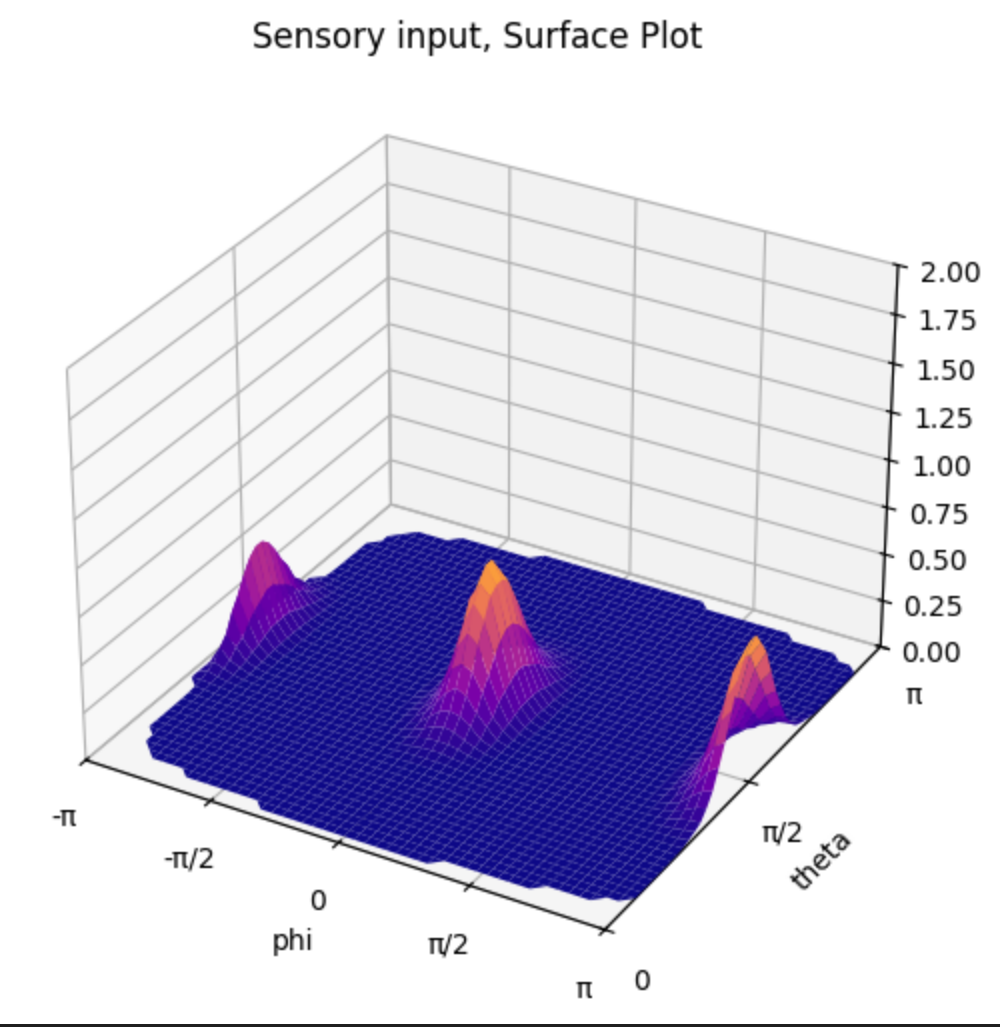
\includegraphics[width=\linewidth]{RAN/RAN_Progress/newer_photos/two_targ_input.png}
    \end{minipage}\hfill
    \begin{minipage}{0.48\linewidth}
        \centering
        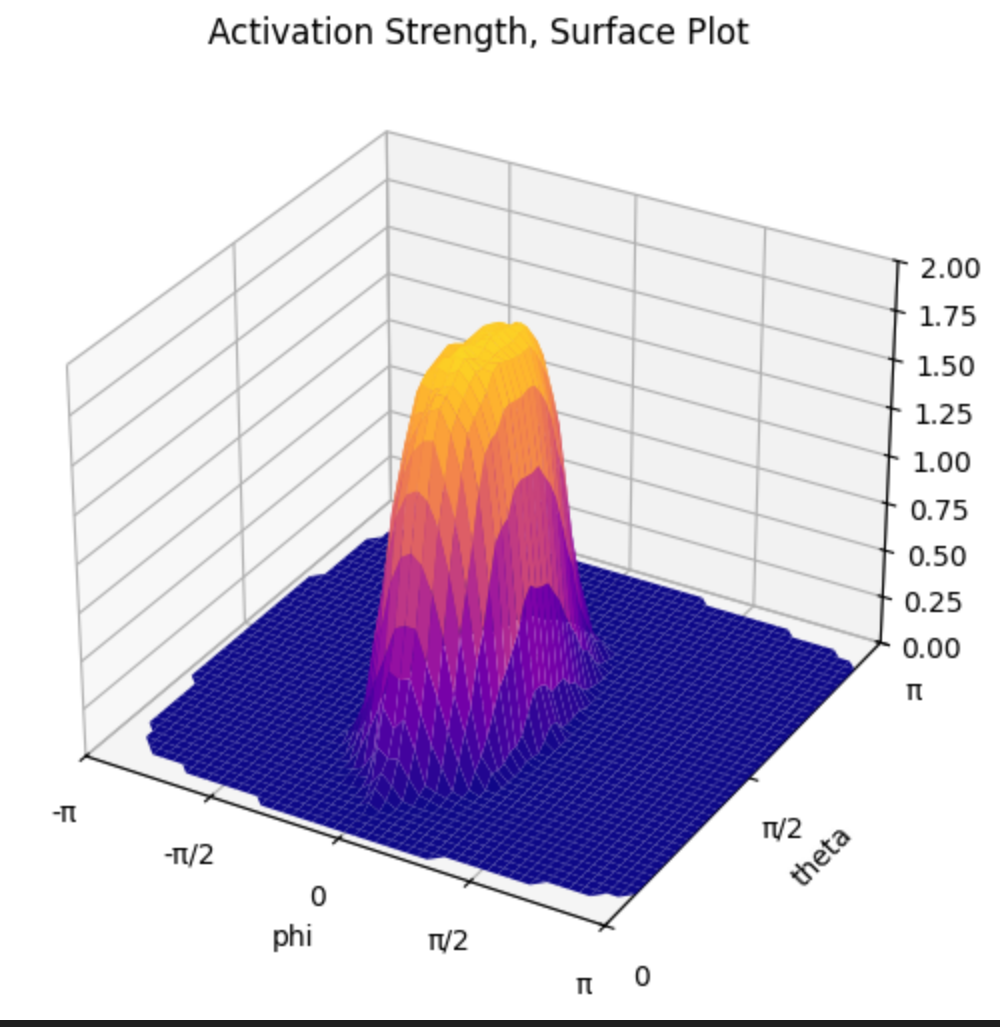
\includegraphics[width=\linewidth]{RAN/RAN_Progress/newer_photos/two_targ_bump.png}
    \end{minipage}
    \caption{Surface plots of sensory input (left) and resulting RAN activation strength (right) for two antipodal targets of equal quality. A stable bump forms over one of the two randomly-selected targets.}
    \label{fig:two_targ_plot}
\end{figure}

In order for a target to be selected, enough time must pass for both global inhibition and inhibition from other nodes for a stable bump to form over one input. Using previously mentioned parameters, 200 timesteps were used for the bump to converge to a target. Below, Figure \ref{fig:2converge} shows a plot of phase error or error in desired angular distance to real angular distance versus each timestep of RAN generation. Note that the timestep axis begins around 40 due to non-meaningful noise produced in initial RAN generation.

\begin{figure}[H]
    \centering
    \includegraphics[width=0.8\linewidth]{RAN//RAN_Progress//Media/2targconvergence.png}
    \caption{Plot of phase error vs RAN update timestep, with error bars present}
    \label{fig:2converge}
\end{figure}

\subsection{Three Target Selection with Equal Qualities}

To test selection between more than two options, three targets of equal quality ($\gamma = 20$) were placed symmetrically around one of the icosphere's 3-fold symmetry axes, each $39^\circ$ from the axis and separated by $120^\circ$ rotations about it. Because the icosphere is unchanged by a $120^\circ$ rotation about this axis, the three targets see identical local node neighborhoods, so no discretization bias favors any one target and only noise decides the winner. For this run, $u = 32$, $\sigma = 1.0$, and $\kappa = 10$ were used.

Figure \ref{fig:three_targ_plot} shows the sensory input (left) and resulting RAN activation (right). Unlike the antipodal two target case, the three targets are close enough together that their input bumps overlap. The network still forms a single bump rather than three, showing that the winner-take-all behavior extends to more than two targets. However, the peak activation (approximately $1.1$) is noticeably lower than in the one and two target cases (approximately $1.8$ to $1.9$), and the bump is less sharply defined. This suggests that the competition between nearby targets is harder to resolve, and further trials are needed to confirm that the bump settles on a single target rather than an average of neighboring targets.

\begin{figure}[H]
    \centering
    \begin{minipage}{0.48\linewidth}
        \centering
        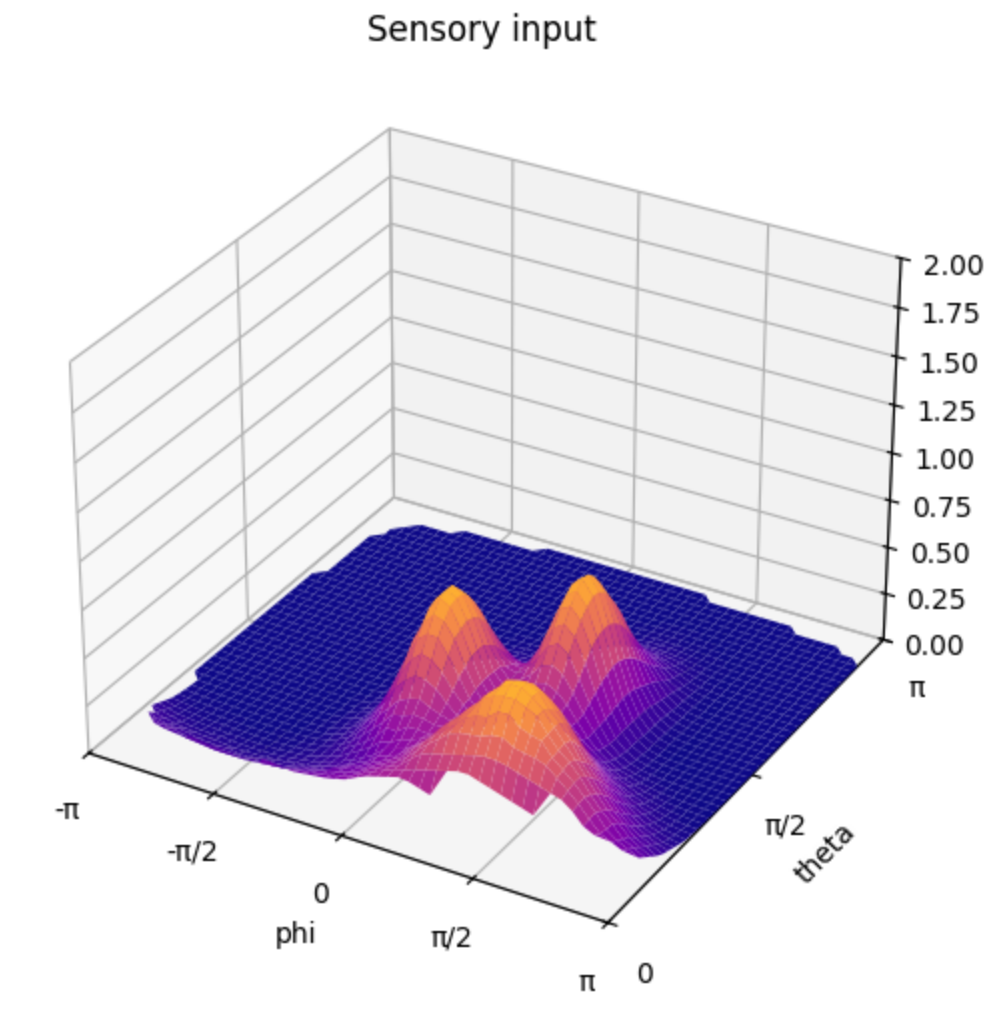
\includegraphics[width=\linewidth]{RAN/RAN_Progress/newer_photos/3_targ_sensory.png}
    \end{minipage}\hfill
    \begin{minipage}{0.48\linewidth}
        \centering
        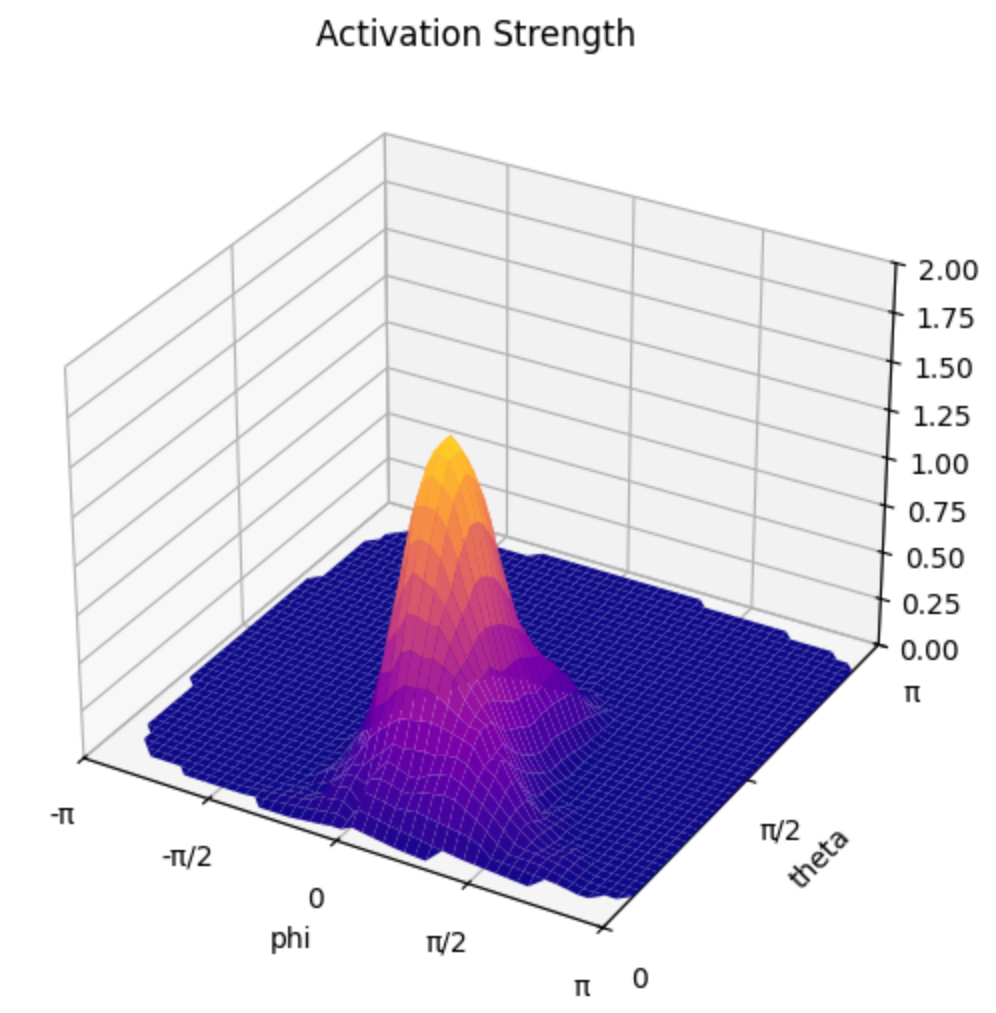
\includegraphics[width=\linewidth]{RAN/RAN_Progress/newer_photos/3_targ_bump.png}
    \end{minipage}
    \caption{Surface plots of sensory input (left) and resulting RAN activation strength (right) for three symmetrically placed targets of equal quality. A single bump forms.}
    \label{fig:three_targ_plot}
\end{figure}

%%%%%%%%%%%%%%%%%%%%%%%%%%%%%%%%%%%%%%%%%%%%%%%%%%%%
\section{Conclusions}

The following lessons were learned during development of the 3D spherical RAN:

\begin{enumerate}
    \item An icosphere with subdivision level $n$ provides near-perfectly equidistant nodes and antipodal symmetry, making it the correct choice for uniform spherical representation.

    \item The connection kernel must be normalized by $1/N$ so that $u_{\text{crit}}$ remains consistent across different resolutions. With the $1/N$ normalization alone, the connection strengths are bounded by $\pm 1/N$ (approximately $\pm 0.0016$ for $N = 642$), which produced the desired behavior with $u = 32$ and the parameters that were used.

    \item Winner-take-all behaviour requires $u > u_{\text{crit}}$ and sufficient noise $\sigma$ for symmetry breaking. At $n=3$ ($N=642$), $\sigma = 1.5$ was found to work reliably when targets were antipodal and their directions were aligned with a node.

    \item Discretization bias is an inherent limitation: a target landing closer to a node receives a stronger peak sensory input $b_{\text{peak}} = e^{\kappa(\cos d - 1)}$, which is monotone decreasing in the node-to-target gap $d$. This bias is amplified by winner-take-all dynamics and can only be reduced by increasing resolution.
    \begin{itemize}
        \item The spherical attractor tends to bias towards targets that are not perfectly centered around a node and that have a shorter, wider bump.
        \item The current theory states that targets which are between multiple nodes (which generate the shorter, narrower input bump) generates sensory input with a greater total energy, that is, the sum of the external sensory input values $b_i$ around the target may be greater than the sum of sensory inputs surrounding targets centered over a node. This causes the ring dynamics to prefer targets that are not centered over nodes.
        \item The solution may be to calculate total integrated input across the Voronoi region of each target, not just the peak value. The target with the greater integrated input would would then be selected. 
        \item One solution that did not work was equalizing only the peaks of the inputs. This means artificially setting the input magnitude of the closest node to the off-center target equal to the input magnitude of the centered target. This is insufficient because it does not account for differences in bump shape.
    \end{itemize}

    \item At 50 Hz real-time integration, subdivision level $n=4$ ($N=2{,}562$) is safe on a modern laptop and borderline on a Raspberry Pi 4. Level $n=3$ ($N=642$) is safe on both.
\end{enumerate}

\section{Appendix A: Code Implementations}
\label{AppendixA}
Icosphere Generation: 
\begin{verbatim}
    import pyvista as pv
    
    icosphere_test = pv.Icosphere(radius=1.0, nsub=Nsub)
    nodes = cartesian_to_polar_3D(icosphere.points.copy())
\end{verbatim}

Kernel Matrix Calculation ($\mathbf{M}$): 
\begin{verbatim}
    for i in range(N):
        for j in range(N):           
            alphas[i, j] = geodesic_distance(nodes[i], nodes[j])
            M[i, j] = J * np.cos(np.pi * np.power((alphas[i,j]/np.pi), v)) 
                * (1/N)
\end{verbatim}


Sensory Input Calculation ($\mathbf{b_i}$):
\begin{verbatim}
    for j in range(len(targets)):
        for i in range(num_nodes):
            alpha = geodesic_distance(sphere_points[i], target_point)
            b[i] += np.exp(kappa * (np.cos(alpha) - 1.0)) 
                * targets[j][QUALITY]
    
    b *= (1/np.sqrt(num_nodes)) 
\end{verbatim}

Euler Integration for Ring Dynamics:
\begin{verbatim}
    y = np.zeros((T, N))
    for t in range(T):
        noise = rand_link_func(y[t], sigma * np.sqrt(dt), 1.0 np.sqrt(N))
        z = z + dt * (-z + np.tanh(u_val * (M @ z) + b - beta) 
            - np.tanh(-beta) + noise) 
        y[t] = z
\end{verbatim} 
*Note that $\mathbf{y}$ stores the entire generation history of the RAN, which is useful for debugging the static generation of the ring attractor. For a continuous or dynamic ring attractor, this term can be omitted and simply the current $\mathbf{z}$ can be used.

%%%%%%%%%%%%%%%%%%%%%%%%%%%%%%%%%%%%%%%%%%%%%%%%%%%%
% --- Bibliography Output ---
\printbibliography 

\end{document}
